% File:      main.tex
% Author:    Zhiying WANG
% Email:     zhiying.wang@tum.de
% Institute: Professur für Satellitengeodäsie
%            Technische Universität München
% Created:   2025-07-24
%
% Description:
%   Main file for thesis
%

\documentclass{tumthesis}
\usepackage{lipsum} % to generate some random content for the template, can be deleted for actual use

% ===============================================================
% Modify the basic information here
\title{Thesis Template}
\subtitle{for \LaTeX}
\author{Zhiying Wang}
\program{M. Sc. Geodesy and Geoinformation/ESPACE}
\chair{Professur für Satellitengeodäsie}
\type{Master's or Bachelor's Thesis}
\supervisorA{Supervisor A}
\supervisorB{Supervisor B}
\supervisorC{If you need to change \\ 
             & the number of supervisors \\ 
             & please go to the tumthesis.cls file}
\submissiondate{01}{10}{2023}
% ===============================================================

\newacronym{gnss}{GNSS}{Global Navigation Satellite System}
\newacronym{gps}{GPS}{Global Positioning System}
\newacronym{leo}{LEO}{Low Earth Orbit}
\makeglossaries

\begin{document}
    \makecover
    \newpage\setcounter{page}{1}\pagenumbering{roman}
% declaration of originality
% Declaration of Originality
\newpage
\thispagestyle{onlypagenum}
\section*{\LARGE Selbstständigkeitserklärung}
Ich versichere hiermit, dass ich die von mir eingereichte Abschlussarbeit selbstständig verfasst und keine
anderen als die angegebenen Quellen und Hilfsmittel benutzt habe.
\par
\vspace{5em}
\begin{tabular*}{\textwidth}{@{}p{10em}@{\extracolsep{\fill}}p{10em}@{}}
    \dotfill & \dotfill \\ 
    \quad Ort, Datum & \quad Unterschrift \\ 
\end{tabular*}

\newpage
\thispagestyle{empty}
\cleardoublepage
\thispagestyle{empty}

% acknowledgements
\newpage
\thispagestyle{onlypagenum}	
% \section*{Acknowledgements}
\vspace*{\fill}
\begin{center}
    \textit{
        Say anything you want
    }
    \par\bigskip
    \textit{
        Paragraph 2 \lipsum[1]
    }
    \par\bigskip
    \textit{
        Paragraph 3 \lipsum[1]
    }
    \par\bigskip
    \textit{
        \dots
    }
\end{center}
\vfill

\newpage
\thispagestyle{empty}
\cleardoublepage
\thispagestyle{empty}
% abstract
\newpage
\thispagestyle{onlypagenum}	
\chapter*{Abstract}
The abstract should be around 250 words. And here is an example for abbreviations: \acrshort{gnss} is the abbreviation for \acrlong{gnss}, and this is the full format abbreviation \acrfull{gnss}. 

\lipsum[1-2]

\newpage
\thispagestyle{empty}
\cleardoublepage
\thispagestyle{empty}

% table of contents
{\hypersetup{linkcolor=black} \tableofcontents \thispagestyle{onlypagenum}}
\cleardoublepage
% list of tables and figures
{\hypersetup{linkcolor=black} \listoftables \thispagestyle{onlypagenum}}
\addcontentsline{toc}{chapter}{List of Tables}
\cleardoublepage
{\hypersetup{linkcolor=black} \listoffigures \thispagestyle{onlypagenum}}
\addcontentsline{toc}{chapter}{List of Figures}
\cleardoublepage
% list of acronym
\setlength{\glsdescwidth}{0.65\linewidth}
\setlength{\glspagelistwidth}{0.2\linewidth}
\addcontentsline{toc}{chapter}{Abbreviations}
{\printglossary[type=\acronymtype,style=long,title={Abbreviations}] \thispagestyle{onlypagenum}}
\cleardoublepage

    % ===============================================================
    % Chapter list, change if you have less or more chapters
    \newpage\setcounter{page}{1}\pagenumbering{arabic}
    \chapter{Introduction}\label{ch:intro}
    \section{Motivation}\label{sec:motiv}
        An example for citation \cite{Hinks2013}. here is an example for abbreviations: \acrshort{gnss} is the abbreviation for \acrlong{gnss}, and this is the full format abbreviation \acrfull{gnss}; \acrshort{gps} is the abbreviation for \acrlong{gps}, and this is the full format abbreviation \acrfull{gps}; \acrshort{leo} is the abbreviation for \acrlong{leo}, and this is the full format abbreviation \acrfull{leo}; 
        
        \lipsum[1]

        An example for figures. 
        \begin{figure}[!ht]
            \centering
            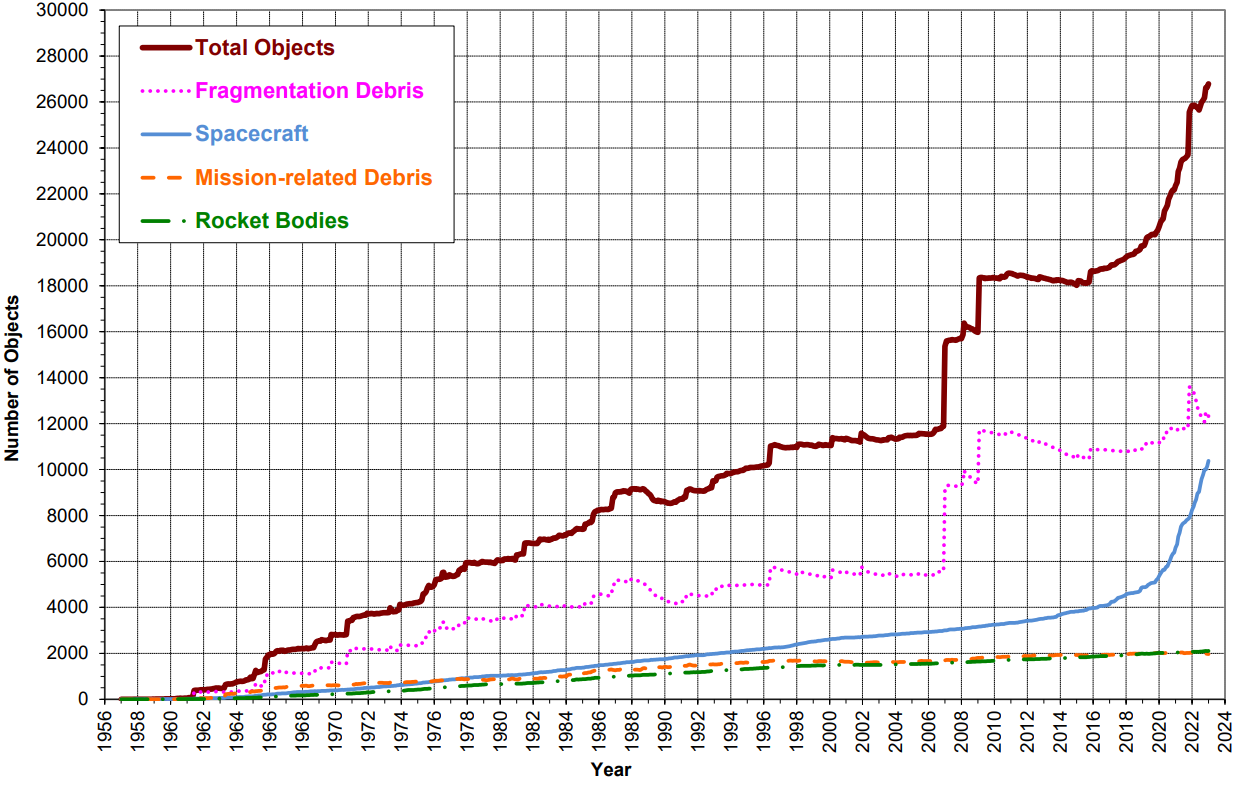
\includegraphics[width=1.0\textwidth]{figures/evo_typ.png}
            \caption[Evolution of number of space objects
            (classified by space object type)]{Evolution of number of space objects
            (classified by space object type)\textsuperscript{\cite{nasa2023}}.}\label{fig:evo_typ}
        \end{figure}
        \begin{figure}[!ht]
            \centering
            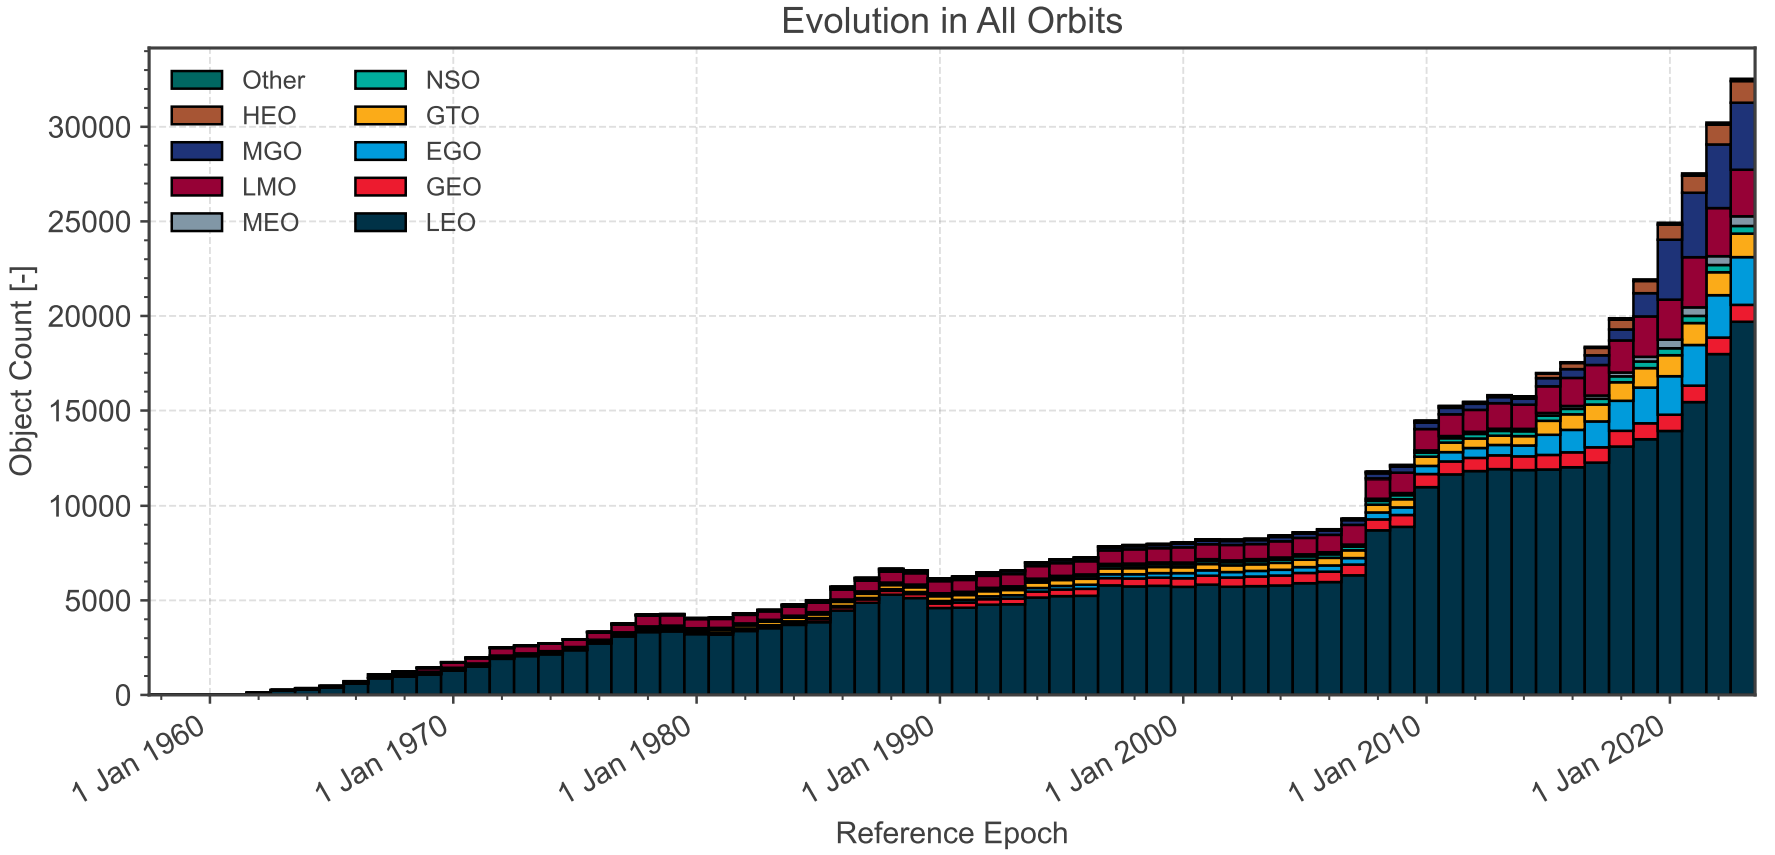
\includegraphics[width=1.0\textwidth]{figures/evo_orb.png}
            \caption[Evolution of number of space objects
            (classified by orbit)]{Evolution of number of space objects
            (classified by orbit)\textsuperscript{\cite{esa2023}}.}\label{fig:evo_orb}
        \end{figure}

    \section{Outline}
        Examples for cross references: 

        Chapter \ref{ch:intro} \lipsum[1]

        Chapter \ref{ch:review} \lipsum[1]
        
        Chapter \ref{ch:theory} \lipsum[1]
        
        Chapter \ref{ch:innovation} \lipsum[1]
        
        Chapter \ref{ch:experiments} \lipsum[1]
        
        Chapter \ref{ch:conclu} \lipsum[1]
        
        Chapter \ref{ch:outlook} \lipsum[1]



    \clearpage{\thispagestyle{empty}\cleardoublepage} % this is to ensure every chapter starts at single page
    \chapter{Related Works}\label{ch:review}
    Review of your references \dots \cite{Hinks2013,esa2023,nasa2023}

    \lipsum[1-3]


    \clearpage{\thispagestyle{empty}\cleardoublepage}
    \chapter{Background}\label{ch:theory}
    An example for table:
    \begin{table}[h!]
        \centering
        \caption{Radiometric quantities in BRDF.}\label{tbl:brdf}
        \begin{tabular}{ l c c l }
            \Xhline{2\arrayrulewidth} 
            \textbf{Quantity} & \textbf{Symbol} & \textbf{Definition} & \textbf{Unit} \\
            \hline \\ [-0.5em]
            Light Power & \(\Phi\) & \(-\) & \(\rm W\) \\ [0.5em]
            Irradiance  & \(E\)    & \(\dfrac{\partial\Phi}{\partial \mathcal{A}}\) & \(\rm W \cdot m^{-2}\) \\ [0.5em]
            Radiance    & \(L\)    & \(\dfrac{\partial^2\Phi}{\partial \omega\partial \mathcal{A}}\) & \(\rm W \cdot m^{-2} \cdot sr^{-1}\) \\ [0.5em]
            \Xhline{2\arrayrulewidth} 
        \end{tabular}
    \end{table}

    An example for equations:
    \begin{equation}
        E_{{\rm obs}(i)} = L_{{\rm obs}(i)} \cdot \omega_{{\rm obs}(i)}
        = C_{\rm sun} \cdot \rho\left(\bm e_{\rm sun}^I , \bm n_{(i)}^I\right) \cdot \left(\bm e_{\rm sun}^I \cdot \bm n_{(i)}^I\right) \dfrac{\mathcal{A}_{(i)} \left(\bm e_{\rm obs}^I \cdot \bm n_{(i)}^I\right)}{d^2}
    \end{equation}

    \lipsum[1-3]
    \clearpage{\thispagestyle{empty}\cleardoublepage}
    \chapter{Innovation}\label{ch:innovation}
    Write about your own creation \dots

    \lipsum[1-3]

    \clearpage{\thispagestyle{empty}\cleardoublepage}
    \chapter{Your Experiments}\label{ch:experiments}
    
    \lipsum[1-3]
    \clearpage{\thispagestyle{empty}\cleardoublepage}
    \chapter{Conclusion}\label{ch:conclu}
\lipsum[1-3]
    \clearpage{\thispagestyle{empty}\cleardoublepage}
    \chapter{Outlook}\label{ch:outlook}
\lipsum[1-3]

    \clearpage{\thispagestyle{empty}\cleardoublepage}
    % ===============================================================

    \newpage
    \addcontentsline{toc}{chapter}{References}
    \renewcommand\bibname{References}
    \bibliographystyle{ieeetr} % We choose the "ieee" reference style
    \bibliography{ref} 
\end{document}
